%\section{Overview of Display Advertising System}
\section{Background}
\label{sec:bg}

%The overall scenario of the display advertising system is illustrated in Figure   \ref{figure_display_ad_scenario}.
In e-commerce sites, such as Alibaba, advertisements are natural goods. In the rest of this paper, without special declaration, we regard ads as goods. Figure \ref{figure_display_ad_scenario} briefly illustrates the running procedure of display advertising system in Alibaba, which consists of two main stages: i) matching stage which generates list of candidate ads relevant to the visiting user via methods like collaborative filtering, ii) ranking stage which predicts CTR for each given ad and then selects top ranked ones.    
%When a user visits the e-commerce site, system
%i) checks his/her historical behavior data;
%ii) generates candidate ads by matching module;
%iii) predicts the click probability (CTR) of each ad and displays top ranked ads under certain ranking score function;
%iv) logs user reactions (click or not) given the displayed ads.
Everyday, hundreds of millions of users visit the e-commerce site, leaving us with lots of user behavior data which contributes critically in building matching and ranking models.
%Rich user historical behavior data contains hint about user interests. 
It is worth mentioning that users with rich historical behaviors contain diverse interests. 
For example, a young mother has browsed goods including woolen coat, T-shits, earrings, tote bag, leather handbag and children's coat recently. These behavior data give us hints about her shopping interests.
When she visits the e-commerce site, system displays a suitable ad to her, for example a new handbag.
Obviously the displayed ad only matches or activates part of interests of this mother. 
In summary, interests of user with rich behaviors are \textsl{\textbf{diverse}} and could be \textsl{\textbf{locally activated}} given certain ads. We show later in this paper making use of these characteristics plays important role for building CTR prediction model.


\begin{figure}
\centering
%\setlength{\belowcaptionskip}{-1cm}
%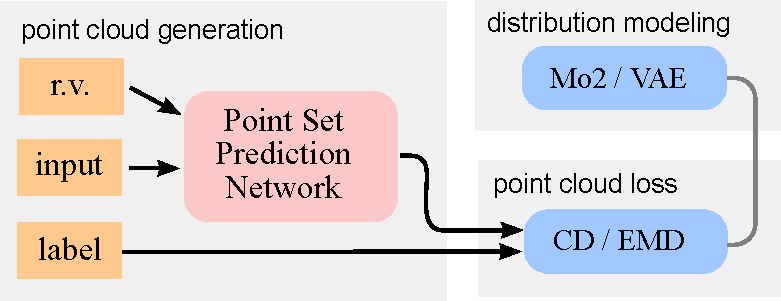
\includegraphics[height=4.5in, width=5in,keepaspectratio]{images/omni/system}
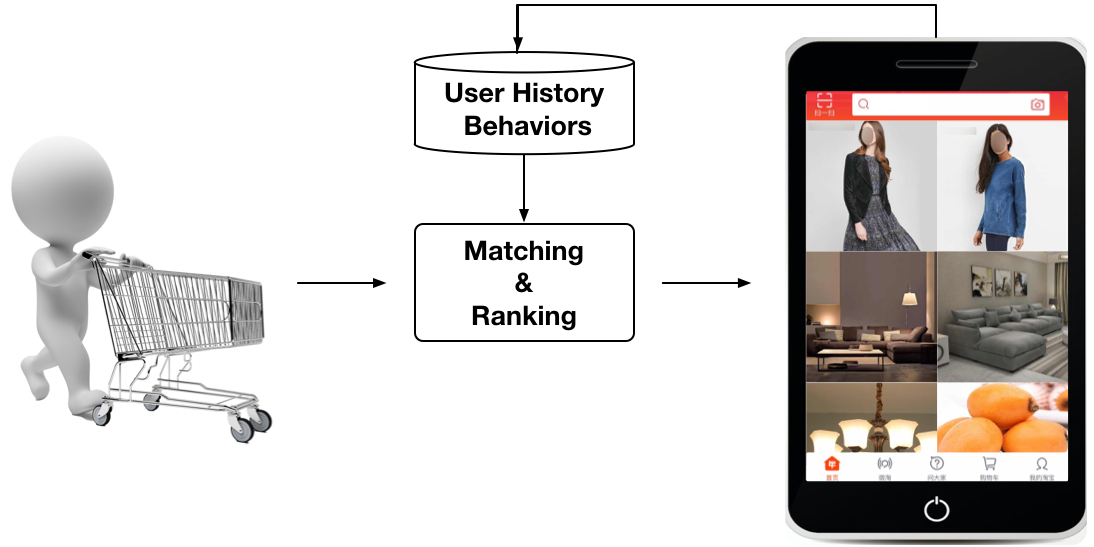
\includegraphics[height=2.5in, width=2.5in,keepaspectratio]{images/omni/sys4.png}
\caption{Illustration of running procedure of display advertising system in Alibaba, in which user behavior data plays important roles.}
\label{figure_display_ad_scenario}
\vspace{-0.4cm}
\end{figure}

 









